\documentclass[tikz,border=8pt]{standalone}
% Shared look for every TikZ diagram. Load with % Shared look for every TikZ diagram. Load with % Shared look for every TikZ diagram. Load with \input{../../tools/tikz-style.tex}
\usepackage[T1]{fontenc}
\usepackage{lmodern}
\renewcommand{\sfdefault}{lmr}  % diagrams use the same serif as the text
\usetikzlibrary{arrows.meta, positioning, shapes.geometric, calc, fit, backgrounds}
\definecolor{cblue}{HTML}{4C78A8}
\definecolor{corange}{HTML}{F58518}
\definecolor{cgreen}{HTML}{54A24B}
\definecolor{cred}{HTML}{E45756}
\definecolor{cpurple}{HTML}{B279A2}
\definecolor{cgrey}{HTML}{6B6B6B}
\tikzset{
  every picture/.style={font=\sffamily, line width=1.2pt},
  box/.style={draw=#1, fill=#1!12, rounded corners=4pt, align=center, inner sep=7pt, minimum height=1.1cm},
  box/.default=cgrey,
  arrow/.style={-{Stealth[length=3mm]}, draw=cgrey, line width=1.4pt},
  title/.style={font=\sffamily\bfseries\Large},
  note/.style={font=\sffamily\small, text=cgrey, align=center},
}
\AtBeginDocument{\hyphenpenalty=10000 \exhyphenpenalty=10000}

\usepackage[T1]{fontenc}
\usepackage{lmodern}
\renewcommand{\sfdefault}{lmr}  % diagrams use the same serif as the text
\usetikzlibrary{arrows.meta, positioning, shapes.geometric, calc, fit, backgrounds}
\definecolor{cblue}{HTML}{4C78A8}
\definecolor{corange}{HTML}{F58518}
\definecolor{cgreen}{HTML}{54A24B}
\definecolor{cred}{HTML}{E45756}
\definecolor{cpurple}{HTML}{B279A2}
\definecolor{cgrey}{HTML}{6B6B6B}
\tikzset{
  every picture/.style={font=\sffamily, line width=1.2pt},
  box/.style={draw=#1, fill=#1!12, rounded corners=4pt, align=center, inner sep=7pt, minimum height=1.1cm},
  box/.default=cgrey,
  arrow/.style={-{Stealth[length=3mm]}, draw=cgrey, line width=1.4pt},
  title/.style={font=\sffamily\bfseries\Large},
  note/.style={font=\sffamily\small, text=cgrey, align=center},
}
\AtBeginDocument{\hyphenpenalty=10000 \exhyphenpenalty=10000}

\usepackage[T1]{fontenc}
\usepackage{lmodern}
\renewcommand{\sfdefault}{lmr}  % diagrams use the same serif as the text
\usetikzlibrary{arrows.meta, positioning, shapes.geometric, calc, fit, backgrounds}
\definecolor{cblue}{HTML}{4C78A8}
\definecolor{corange}{HTML}{F58518}
\definecolor{cgreen}{HTML}{54A24B}
\definecolor{cred}{HTML}{E45756}
\definecolor{cpurple}{HTML}{B279A2}
\definecolor{cgrey}{HTML}{6B6B6B}
\tikzset{
  every picture/.style={font=\sffamily, line width=1.2pt},
  box/.style={draw=#1, fill=#1!12, rounded corners=4pt, align=center, inner sep=7pt, minimum height=1.1cm},
  box/.default=cgrey,
  arrow/.style={-{Stealth[length=3mm]}, draw=cgrey, line width=1.4pt},
  title/.style={font=\sffamily\bfseries\Large},
  note/.style={font=\sffamily\small, text=cgrey, align=center},
}
\AtBeginDocument{\hyphenpenalty=10000 \exhyphenpenalty=10000}

\begin{document}
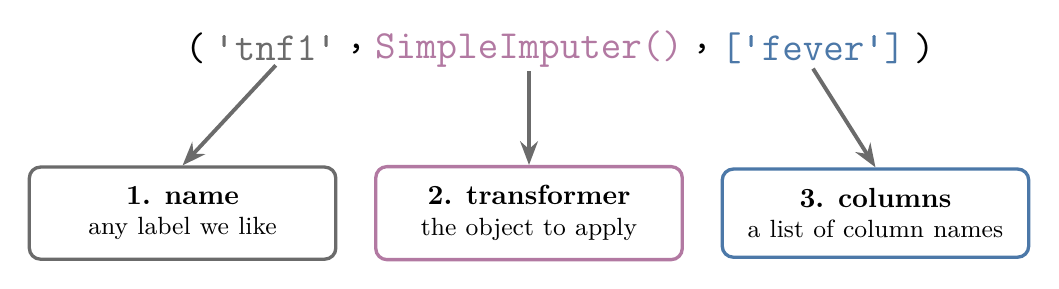
\begin{tikzpicture}
  \node[font=\ttfamily\Large, inner sep=1pt] (p0) {(};
  \node[font=\ttfamily\Large, text=cgrey, right=0pt of p0, inner sep=1pt] (n) {\textquotesingle{}tnf1\textquotesingle{}};
  \node[font=\ttfamily\Large, right=0pt of n, inner sep=1pt] (c1) {, };
  \node[font=\ttfamily\Large, text=cpurple, right=0pt of c1, inner sep=1pt] (t) {SimpleImputer()};
  \node[font=\ttfamily\Large, right=0pt of t, inner sep=1pt] (c2) {, };
  \node[font=\ttfamily\Large, text=cblue, right=0pt of c2, inner sep=1pt] (c) {[\textquotesingle{}fever\textquotesingle{}]};
  \node[font=\ttfamily\Large, right=0pt of c, inner sep=1pt] {)};
  \node[box=cgrey, fill=white, text width=3.4cm] (bn) at ($(t.south)+(-4.4,-1.8)$) {\textbf{1. name}\\[-1pt]\small any label we like};
  \node[box=cpurple, fill=white, text width=3.4cm] (bt) at ($(t.south)+(0,-1.8)$) {\textbf{2. transformer}\\[-1pt]\small the object to apply};
  \node[box=cblue, fill=white, text width=3.4cm] (bc) at ($(t.south)+(4.4,-1.8)$) {\textbf{3. columns}\\[-1pt]\small a list of column names};
  \draw[arrow] (n.south) -- (bn.north);
  \draw[arrow] (t.south) -- (bt.north);
  \draw[arrow] (c.south) -- (bc.north);
\end{tikzpicture}
\end{document}
